% ============================================
\section{Opis problemu}
% ============================================

\begin{frame}[t]{Stan kalkulatorów emerytalnych na 2025 rok}
\begin{itemize}
  \item Narzędzia dostępne publicznie wymagają od użytkownika szeregu wejściowych parametrów
  \pause
  \item Wielu użytkowników nie ma wiedzy, jak realistycznie je oszacować
  \pause
  \item Skutkiem są wyniki obarczone dużą niepewnością lub po prostu: rezygnacja
  z użycia narzędzia przez potencjalnych użytkowników
\end{itemize}
\end{frame}

\begin{frame}[t]{Stan kalkulatorów emerytalnych na 2025 rok}

\includegraphics[width=.8\textwidth]{img/zus_calculator_01}
\end{frame}

\begin{frame}[t]{Stan kalkulatorów emerytalnych na 2025 rok}
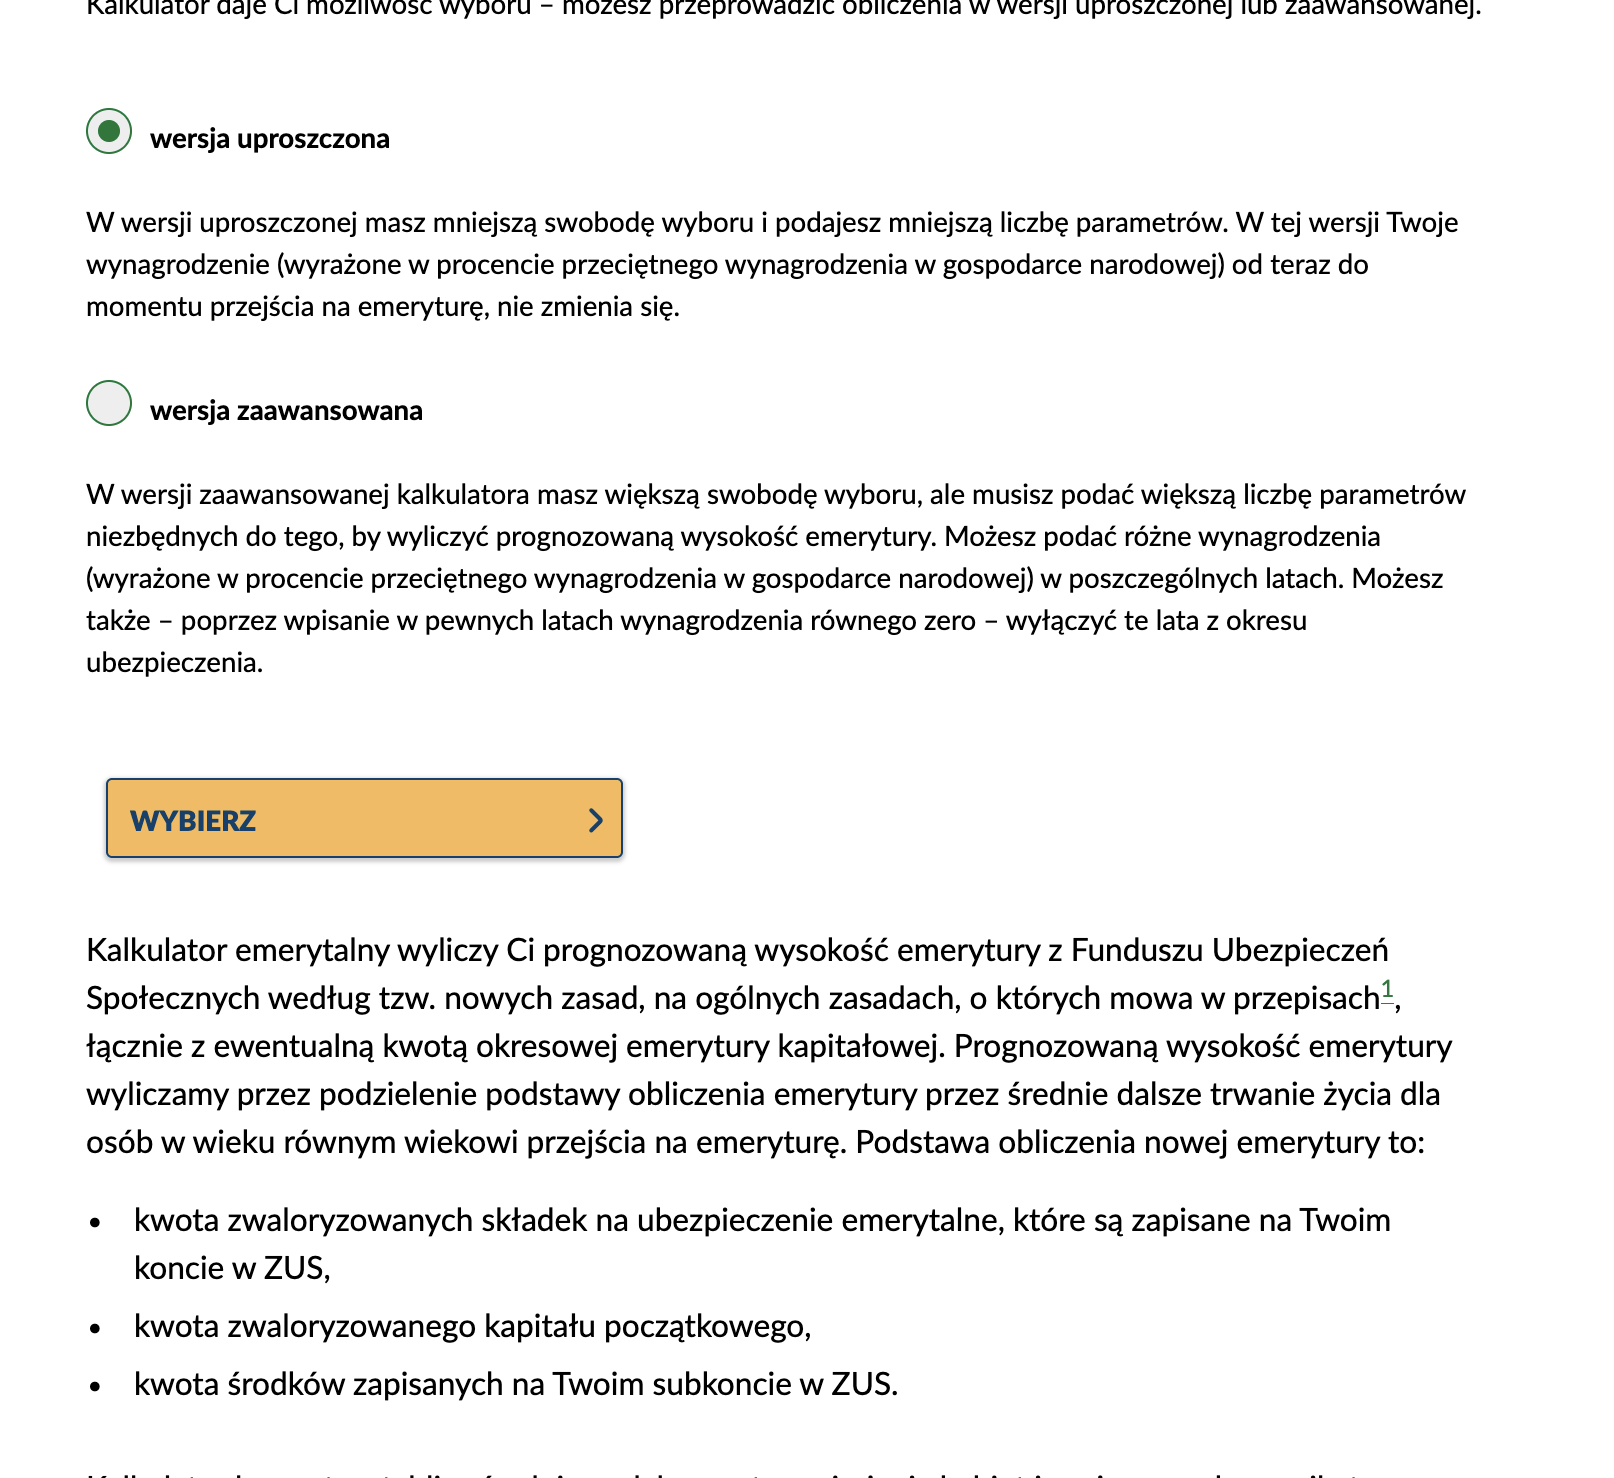
\includegraphics[width=.8\textwidth]{img/zus_calculator_02}
\end{frame}

\begin{frame}[t]{Stan kalkulatorów emerytalnych na 2025 rok}
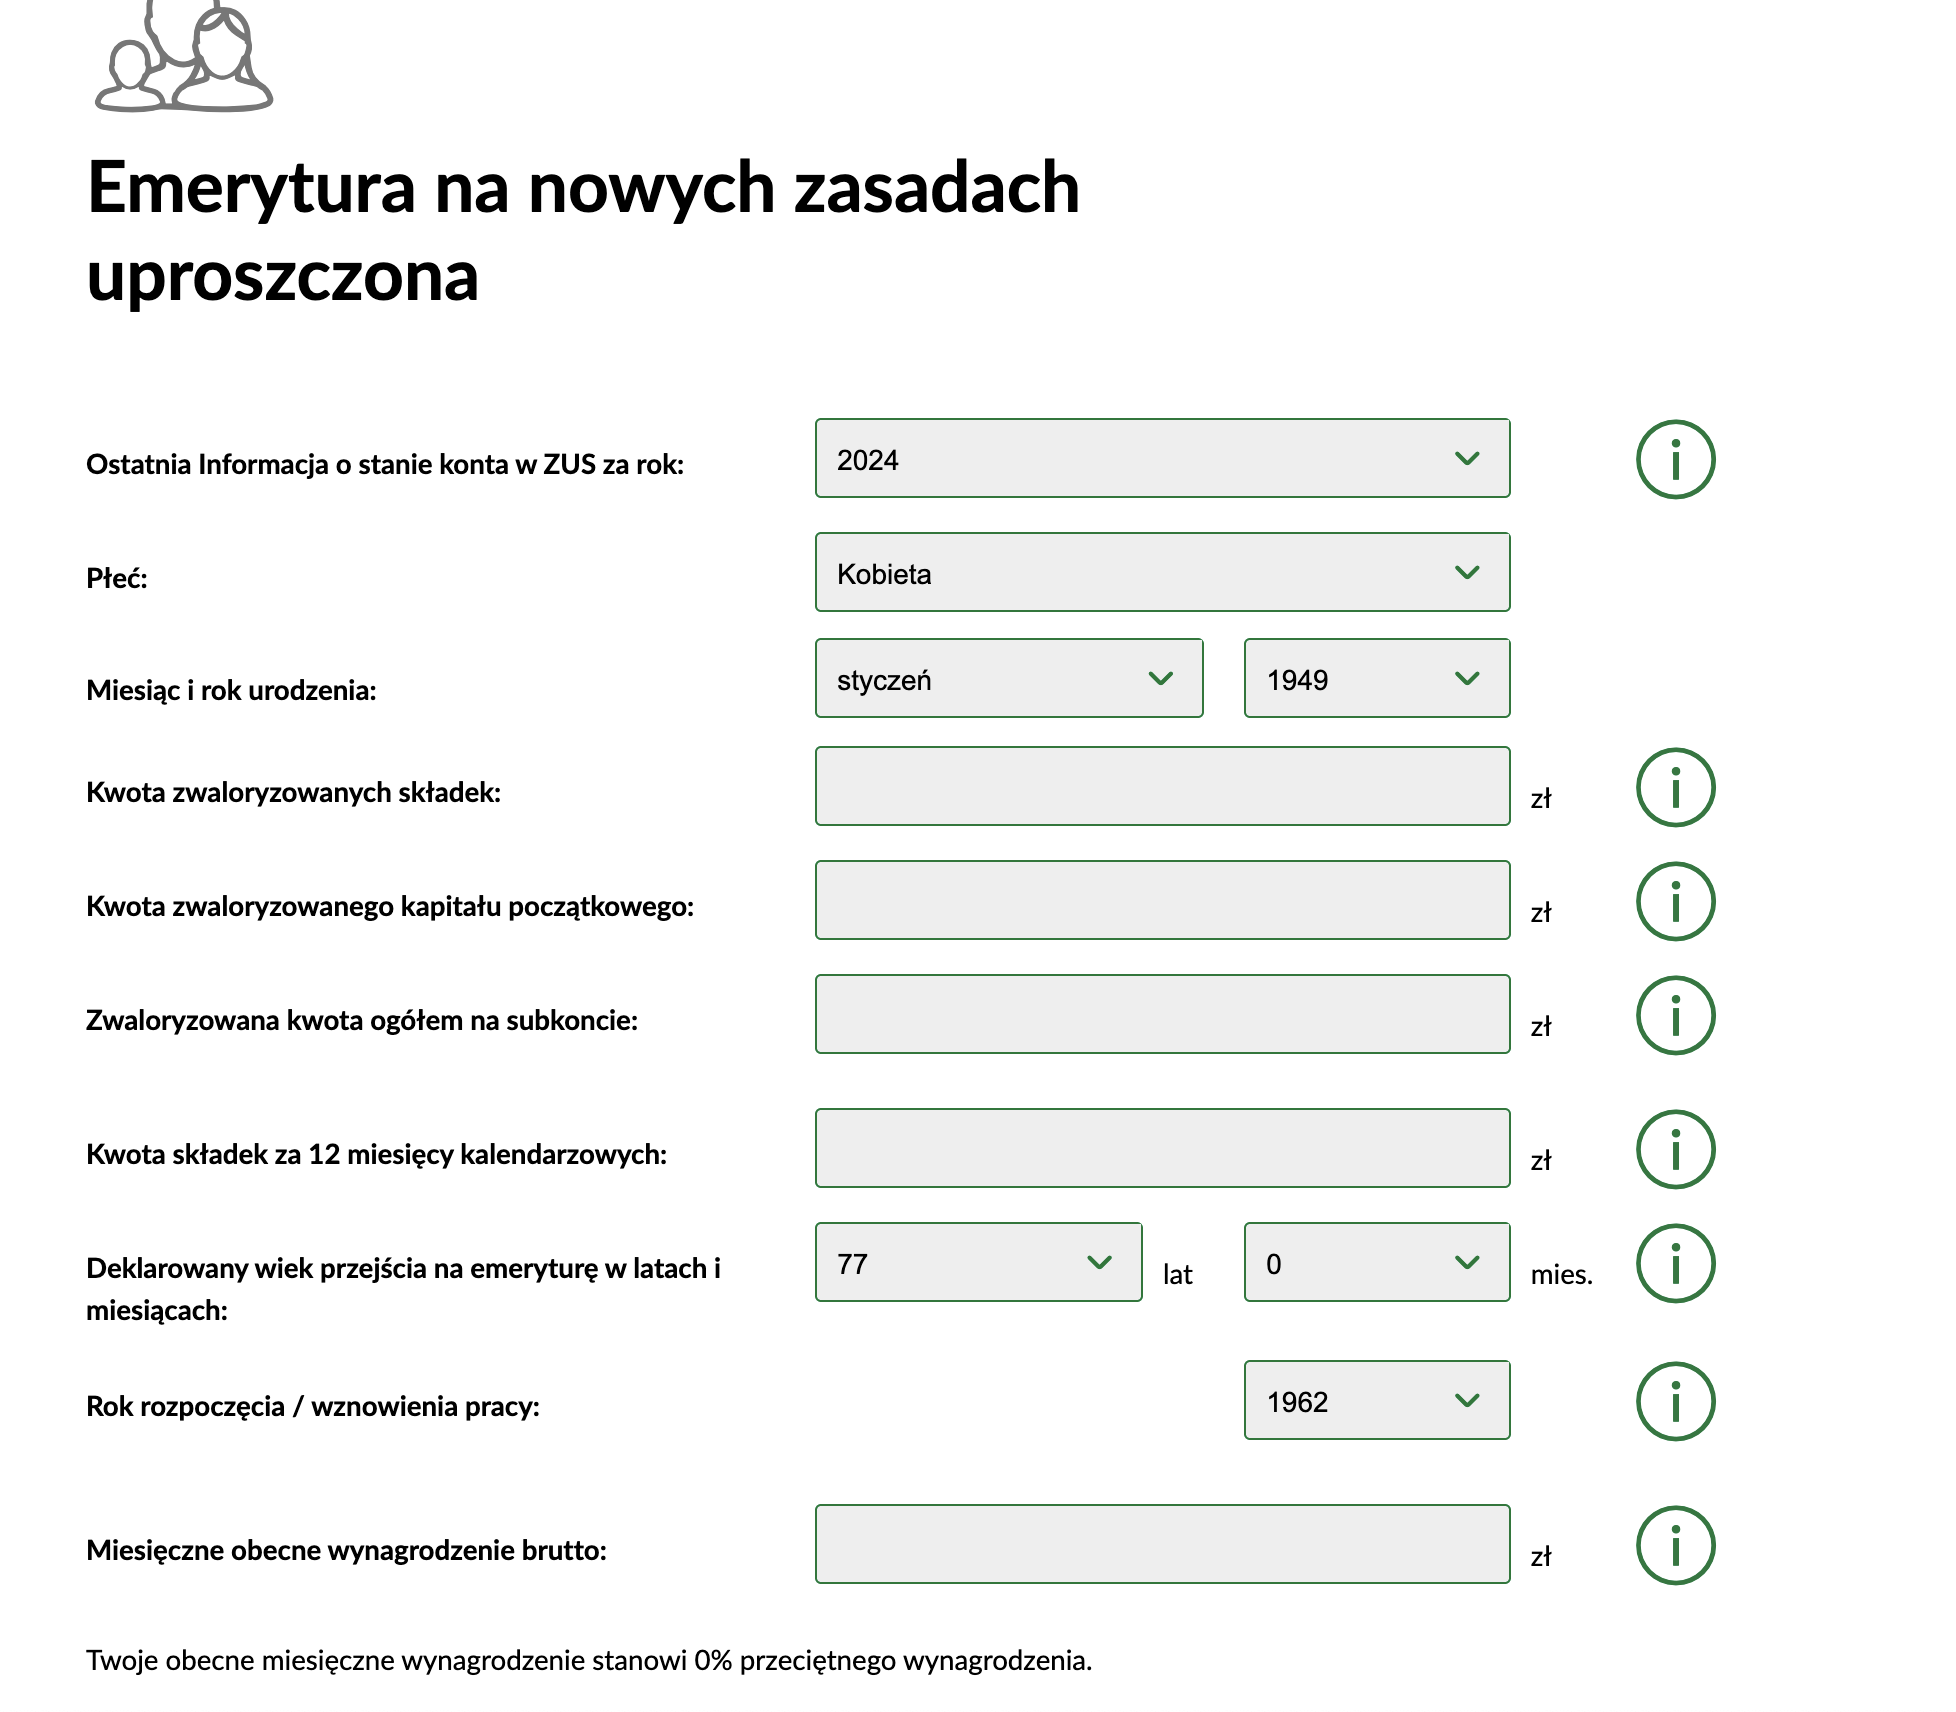
\includegraphics[width=.8\textwidth]{img/zus_calculator_03}
\end{frame}
